\section{논의}\label{sec:discussion}

\subsection{언제 이벤트 커널이 우세한가}\label{sec:when}

식~(\ref{eq:costmodel})에 V장의 적합값($\alpha\approx0.032$,
$\beta\approx1.09$)을 넣으면 조밀 경로와의 손익분기 밀도는
$\rho^{*}=(1-\alpha)/\beta\approx0.89$다
(그림~\ref{fig:costmodel}). 두 레이어로 정한 1차 모델의 외삽이므로
정밀값이 아니라 규모 추정으로 읽어야 하지만
(두 레이어는 $r$$\cdot$채널 수$\cdot$가중치 상주 위치가 다르고,
밀도는 전수 호스트 평균$\cdot$시간비는 보드 8장 표본이다), 함의는
규모 수준에서도 뚜렷하다: \textbf{활성의 약 90\%가 발화하기
전까지는 이벤트 커널이 우세하다}. 학습된 SNN의 은닉층 발화율이 통상 수 퍼센트대임을
고려하면, SNN의 실질 동작 영역 전체가 희소 우세 구간 안에 있다.
역으로 이 모델은 우세의 끝도 알려 준다: 본 파이프라인의 입력층은
rate coding 탓에 밀도 47.7\%로 예외적으로 높고, 그래서 이득이
1.8배에 그치며 최적화 후 병목이 그리로 이동했다
(V장). 밀도를 코딩 수준에서 낮추는 것 --- 예컨대 시간
코딩 --- 이 커널 개선과 직교하는 다음 지렛대라는 뜻이다.

\begin{figure}[htbp]
\centering
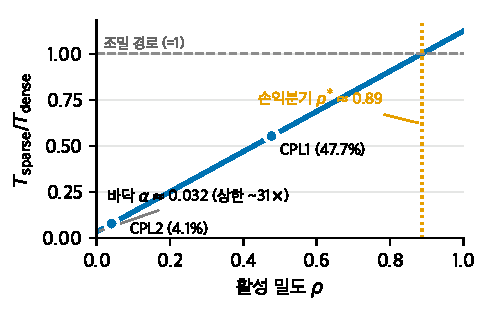
\includegraphics[width=0.9\linewidth]{figures/fig_costmodel.pdf}
\caption{시간비 $T_{\mathrm{sparse}}/T_{\mathrm{dense}}$ 대 활성
밀도 $\rho$. 실측 두 점(CPL1$\cdot$CPL2)으로 정한
식~(\ref{eq:costmodel})의 1차 모델은 손익분기
$\rho^{*}\!\approx\!0.89$와
이득 상한 $1/\alpha\!\approx\!31\times$를 시사한다.}
\label{fig:costmodel}
\end{figure}

\subsection{무엇을 회수했고 무엇이 남는가}

본 연구가 회수한 것은 이벤트 구동성의 \emph{산술적} 몫 --- 0
피연산자의 로드$\cdot$곱셈 제거 --- 이다. 뉴로모픽 하드웨어가
추가로 제공하는 몫, 즉 클럭 없는 비동기 실행$\cdot$이벤트 기반
전력 게이팅$\cdot$메모리-연산 병치는 소프트웨어로 회수되지 않는다.
따라서 본 결과는 뉴로모픽 칩의 대체가 아니라, ``전용 실리콘 없이도
회수 가능한 몫이 정확히 얼마인가''에 대한 한 실측 데이터점이다.
같은 이유로 본 논문은 지연시간을 보고하며, 에너지는 별도 계측
없이 지연 비례 추정 이상을 주장하지 않는다.

방법론 측면에서는 두 가지가 이 결과를 가능하게 했다.
첫째, \emph{의미 보존 계약}(4.1절)이다. 비트 동일성이 상시
검증되는 불변식이었기에 im2col 제거$\cdot$전치$\cdot$블로킹 같은
공격적 재배열을 주저 없이 시도할 수 있었고, k3의 퇴행 같은 실패도
정확성 불안 없이 성능 문제로만 다룰 수 있었다. 둘째, \emph{측정
우선 진단}(III장)이다. 마이크로벤치마크가 지목한 병목을 워크로드
절제로 반증하지 않았다면, 페치 최적화에 노력이 소진되었을 것이다.

\subsection{한계}\label{sec:limits}

본 연구의 한계를 명시한다. (i) 단일 모델$\cdot$단일 보드의
실측이다. 비용 모델이 형상 의존 파라미터를 흡수하지만, 다른
네트워크$\cdot$다른 Cortex-M 등급에서의 $\alpha,\beta$는 재적합이
필요하다. (ii) 체크섬 검증의 범위는 실행된 경로에
국한된다(V장). (iii) 정수 구현의 전체 테스트셋 정확도를 보드에서
직접 실측하지는 못했다 --- 선행 연구와 공유하는 한계다. (iv) 입력층
밀도(47.7\%)는 rate coding의 산물로, 코딩 방식을 바꾸면 이득
분포도 달라진다. (v) 에너지를 직접 계측하지 않았다.
